\chapter{User documentation}
\label{chap:user_docs}

In this chapter, the user documentation is presented. Firstly, the deployment process is described. We distinguish between two types of users, regular users and developers. We expect regular users to use PrankWeb without modifying the existing code. On the other side, we expect developers to add their own plug-ins or make other changes to the existing architecture. For this purpose, we describe a guide for both types of users.

\section{Deployment}
\label{sec:deployment}

This section describes how to deploy the application. The preferred way is to deploy PrankWeb using Docker.

\subsection{Docker deployment}
\label{subsec:docker_deployment}

Firstly, Docker and Docker Compose need to be installed\footnote{Downloadable from the official website at \url{https://docs.docker.com/get-docker/}}. 

After installing Docker, the PrankWeb repository needs to be cloned, preferably using Git\footnote{Downloadable from the official website at \url{https://git-scm.com/downloads}}.

\begin{enumerate}
    \item Create a directory for the PrankWeb repository and navigate to it.
    \item Clone the repository using the following command:
    \begin{lstlisting}[language=clean]
    git clone https://github.com/cusbg/prankweb.git .
    \end{lstlisting}
    \item Create directories for each of the volumes.
    \item Create mounts for each of the volumes in the \texttt{docker-compose.yml} file. The mounts are created as follows, simply update the \texttt{/tmp/} paths to the paths of the directories created in the previous step:
    \begin{lstlisting}
    docker volume create --name prankweb_rabbitmq --opt type=none --opt device=/tmp/rabbitmq --opt o=bind

    docker volume create --name prankweb_conservation --opt type=none --opt device=/tmp/conservation --opt o=bind

    docker volume create --name prankweb_predictions --opt type=none --opt device=/tmp/predictions --opt o=bind

    docker volume create --name prankweb_services --opt type=none --opt device=/tmp/services --opt o=bind

    docker volume create --name prankweb_docking --opt type=none --opt device=/tmp/docking --opt o=bind
    \end{lstlisting}
    \item Optionally, create a \texttt{.env} file to change the default variables defined in the \texttt{docker-compose.yml} file. Notice that UID and GID need to have the write permissions to the directories created in the previous steps.
    \item Build the Docker images using the following command:
    \begin{lstlisting}
    docker-compose build
    \end{lstlisting}
    \item Optionally, download the conservation database (keep in mind that this database is large, around 30 GB):
    \begin{lstlisting}
    docker-compose run --rm executor python3 /opt/hmm-based-conservation/download_database.py
    \end{lstlisting}
    \item Start the containers using the following command:
    \begin{lstlisting}
    docker-compose up
    \end{lstlisting}
\end{enumerate}

The application is now accessible at \url{http://localhost:8020/}.

Although the main deployment process will not change much, the best way to get the current information is to refer to the official documentation at \url{https://github.com/cusbg/p2rank-framework/wiki/PrankWeb-deploy-with-Docker}.

\subsection{Local deployment}
\label{subsec:local_deployment}

Local deployment is not recommended, as the support for some components is limited.

The only component that is developed better locally is the frontend (when not considering backend API changes). To run the frontend locally, firstly clone the repository as described in \ref{subsec:docker_deployment}. Then, navigate to the \texttt{frontend} directory.

It is recommended to have a look at the \texttt{server/configuration.js} file to set up the proxy server that will serve potential calls. The proxy service should be running, it is possible to use the default PrankWeb website at \url{https://prankweb.cz}.

This is the default configuration:
\begin{lstlisting}
    // This configuration is used only in develop mode.
    module.exports = {
        // Port used to run-develop instance.
        "port": 8075,
        // Use this to server data from files. Thus, you can develop
        // frontend without the need to run another component.
        //"proxy-directory": "../../data/database/",
        // Use the option below to proxy commands to the task runner instance.
        // This allows you to run tasks or connect to an existing instance (https://prankweb.cz).
        "proxy-service": "https://prankweb.cz",
    }
\end{lstlisting}

After setting up the proxy server, the frontend npm modules need to be installed. This can be done using the following command:
\begin{lstlisting}
    npm ci
\end{lstlisting}

Then, it is possible to run the frontend using the following command:
\begin{lstlisting}
    npm run dev
\end{lstlisting}

The frontend is now accessible at \url{http://localhost:8075/} (with the port specified in the configuration file).

Some of the tools from the executors like P2Rank may work from the command line as used in the Python scripts or Dockerfiles, for more information refer to those.

Official documentation for the local deployment is available at \url{https://github.com/cusbg/p2rank-framework/wiki/PrankWeb-deploy-for-development}.


\section{Regular user}
\label{sec:regular_user}

Regular users are not expected to modify the existing code. The following section describes how to use the application.

The only requirement is to have a web browser with JavaScript and WebGL support.

Firstly, select a protein structure for the analysis in an input form. Expected inputs are either a protein structure code for experimental structures from the RCSB PDB, a custom PDB or mmCIF file, or a UniProt ID of a predicted structure. It is possible to use conservation data from the HMM-based conservation database to provide more information for the prediction. For experimental structures, it is possible to restrict the prediction just to specified chains. The input form is shown in \cref{fig:input_form}.

\begin{figure}[ht]
    \centering
    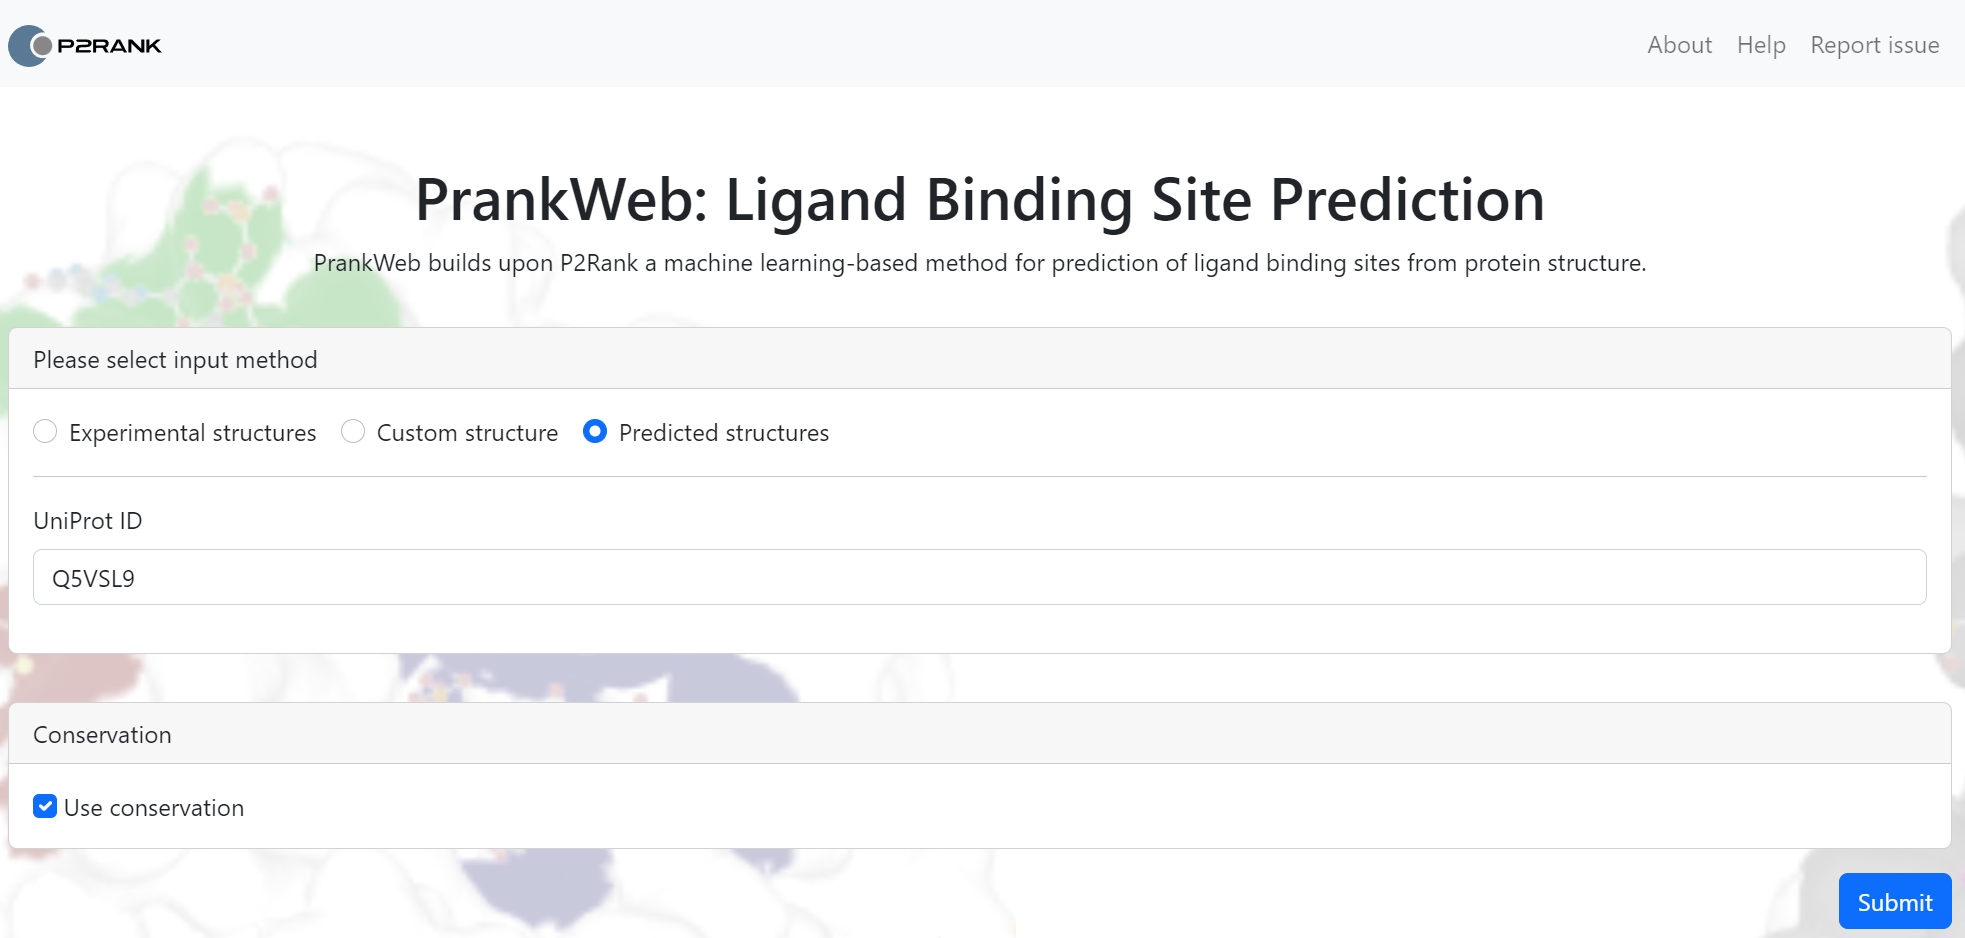
\includegraphics[width=\textwidth]{img/pw_introsite.png}
    \caption{Input form for the PrankWeb application.}
    \label{fig:input_form}
\end{figure}

Then, a prediction task is created and sent to the backend. During the prediction, a log of the task is shown. After the task finishes, the viewers are shown. The PrankWeb viewers are shown in \cref{fig:prankweb_viewers}.

\begin{figure}[ht]
    \centering
    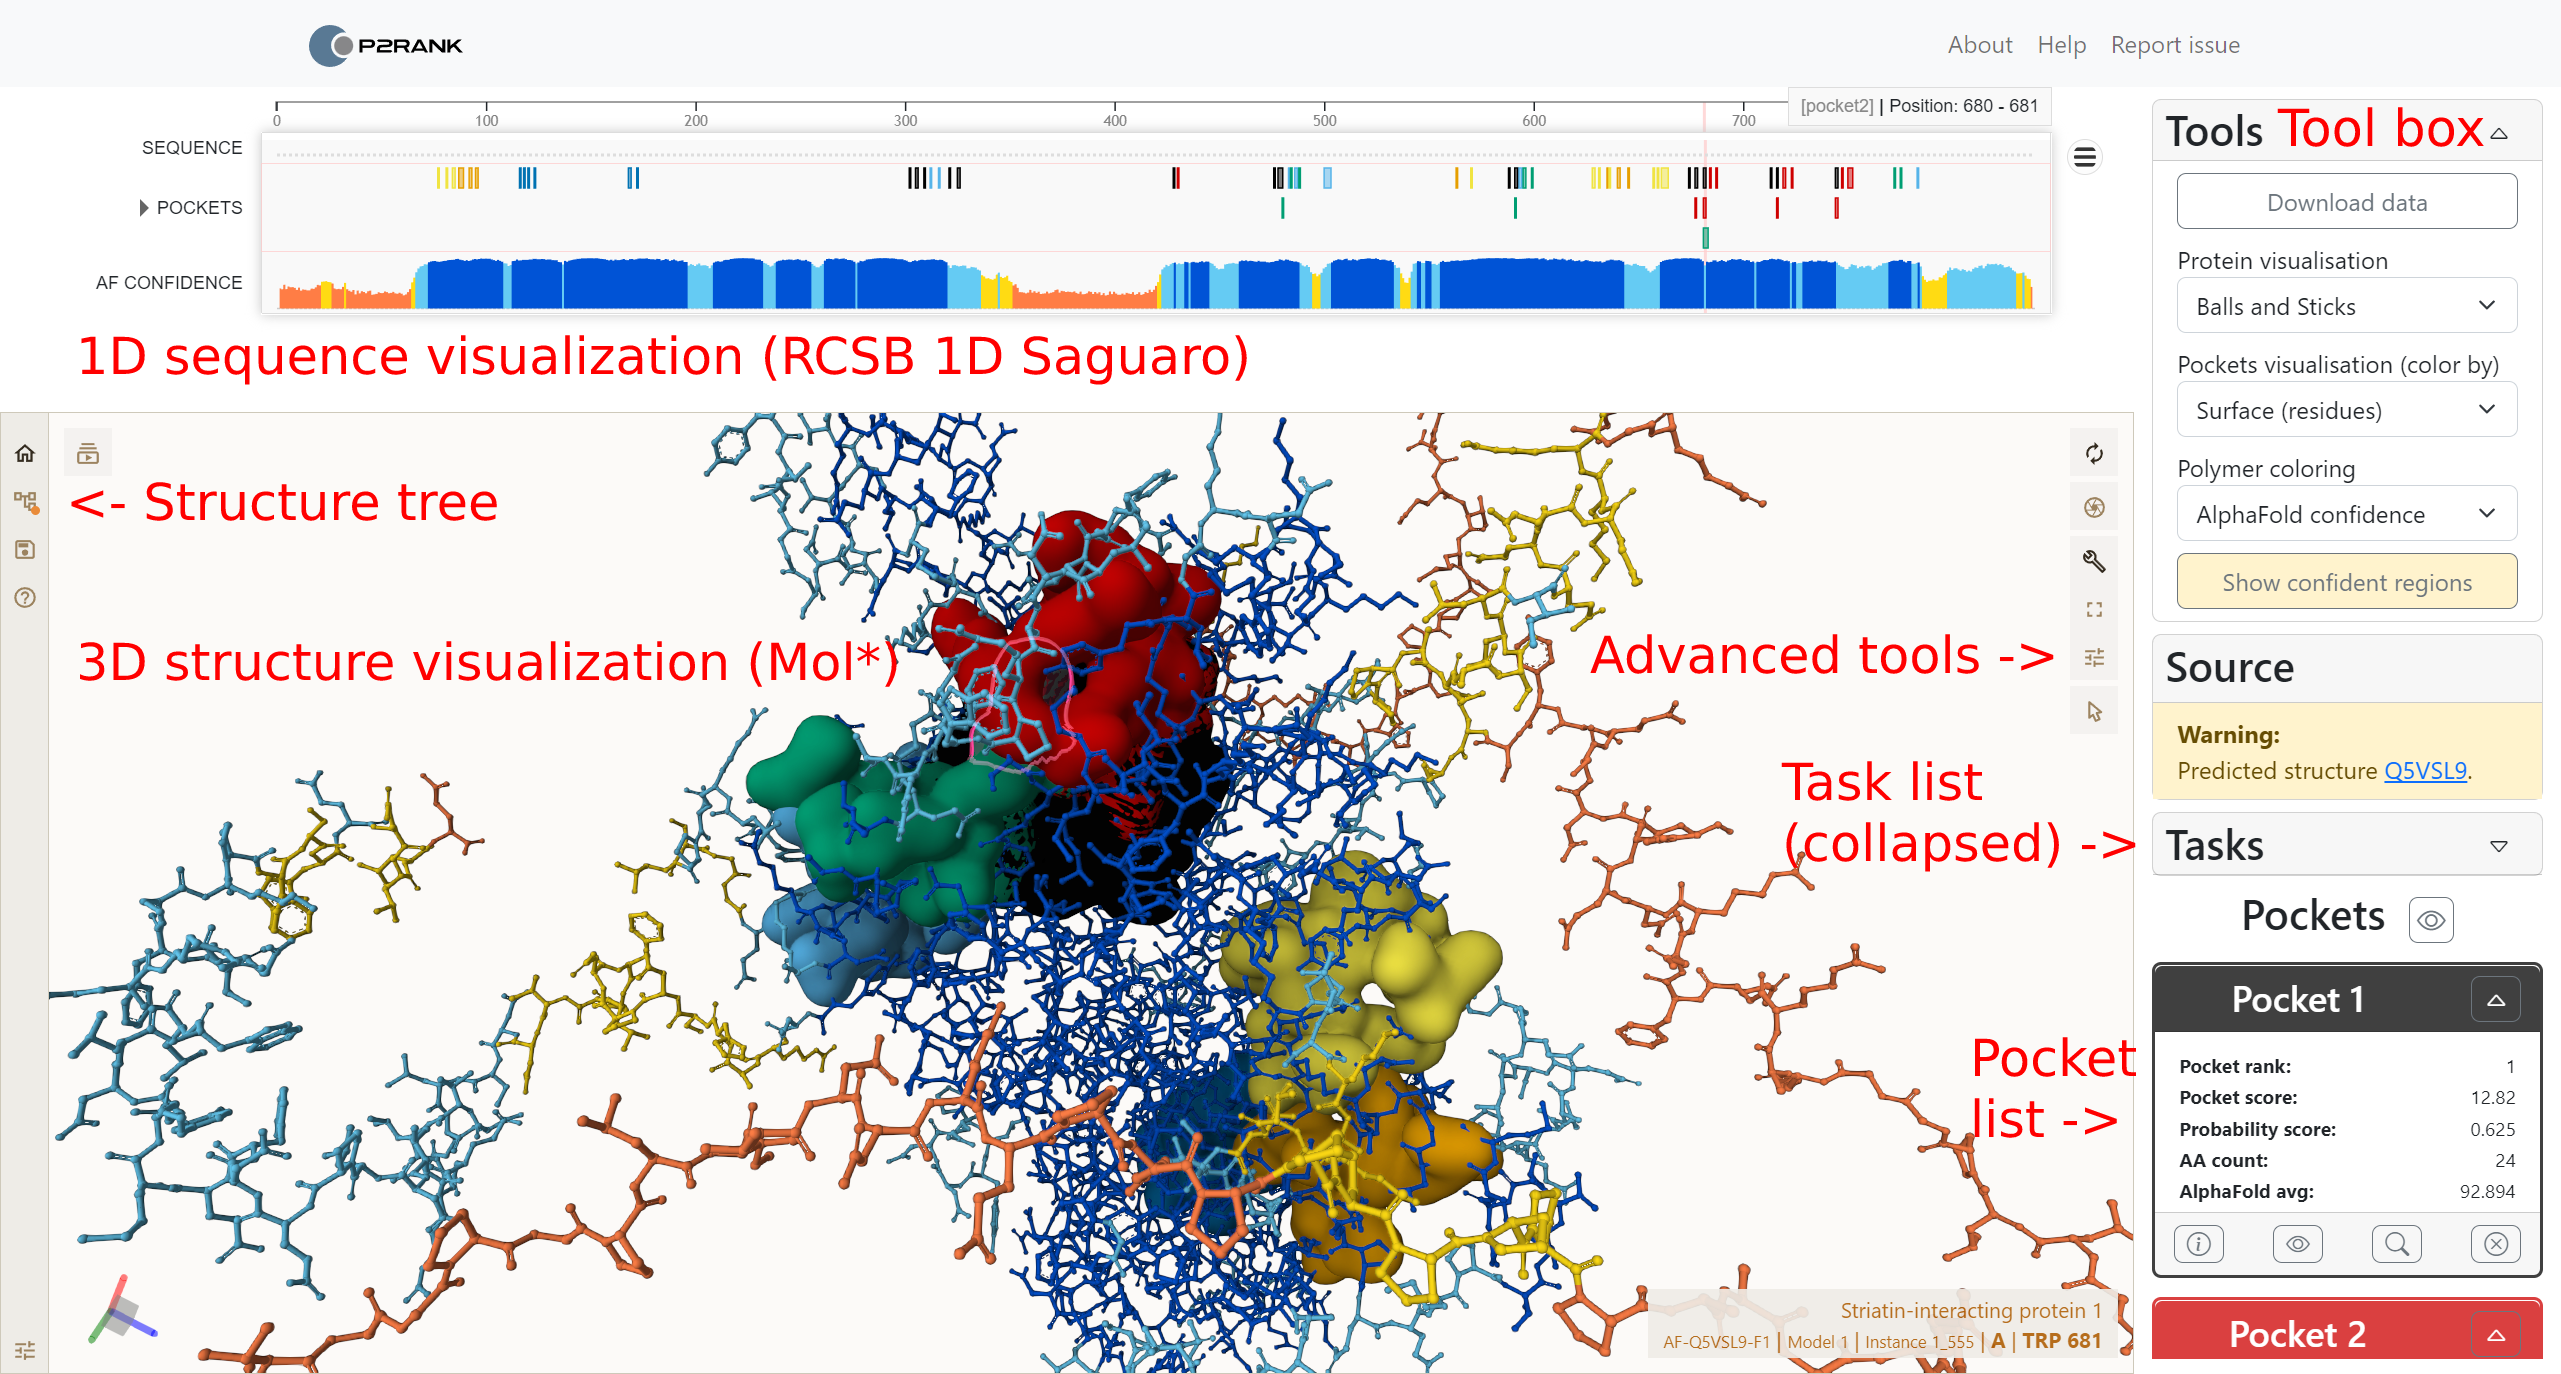
\includegraphics[width=\textwidth]{img/pw_predict.png}
    \caption{The main PrankWeb interface showing visualizations of the \texttt{P21802} UniProt structure.}
    \label{fig:prankweb_viewers}
\end{figure}

Once the protein visualization is loaded, three main panels appear - sequence visualization, structural visualization and the pocket panel.

On the left side, both viewers visualizing the structure are shown. There is the RCSB 1D Saguaro Viewer on the top for the 1D visualization of the properties of the structure and predicted binding sites. On the bottom, we may see the Mol* viewer for the 3D visualization of the structure and pockets. 

By default, the protein surface is displayed, and individual pocket areas are highlighted with different colors. Ligands may be displayed as separate molecules as well, if available. It is possible to change the colors of the protein based on the conservation or plDDT score in the toolbox on the right side. For conservation coloring, darker residues depict a higher score. For plDDT coloring, the colors are defined by the AlphaFold confidence score \cite{david2022alphafold}.

The 3D structure may be rotated by dragging the mouse while holding the left mouse button. The zoom is controlled by the mouse wheel or by pinching on touch devices. For moving the protein structure, the right mouse button may be used. The structure may be reset to the default position by clicking the reset button in the top right corner of the 3D viewer.

Mol* provides more features for visualization. Using the buttons in the top-right corner, one can:

\begin{itemize}
    \item Reset the camera.
    \item Create a snapshot of the current visualization.
    \item Toggle the advanced control panel.
    \item Toggle full-screen mode.
    \item Setup the scene such as the visualization background or the field of view.
    \item Toggle the selection mode.
\end{itemize}

After toggling the advanced control panel, the following may be done:

\begin{itemize}
    \item Work with the structure and download it.
    \item Toggle the state tree and thus toggle multiple of the available representations.
    \item Save the current plugin state.
    \item View the help panel.
\end{itemize}

For more information, please refer to the Mol* documentation at the official website\footnote{The Mol* documentation is available at \url{https://molstar.org/viewer-docs/}}.

The RCSB 1D Saguaro Viewer displays the protein sequence. It does the following:

\begin{itemize}
    \item All chains are concatenated into a single sequence and shown at once.
    \item Colored rectangles depict the predicted binding sites. The colors are the same as in the 3D viewer.
    \item Real binding sites are shown as well. As real binding sites, we consider any residues within 4 \AA{} from a ligand atom.
    \item If available, conservation and plDDT scores are shown as well.
\end{itemize}

The Mol* viewer and the 1D Saguaro Viewer are synchronized. This means that when hovering over a residue in the 1D viewer, the corresponding residue in Mol* is highlighted. The same applies to the 3D viewer. When hovering over a residue in Mol*, the corresponding residue in the 1D viewer is highlighted. Furthermore, after clicking on a residue in the 1D viewer, Mol* focuses on the corresponding residue.

The right panel consists of a toolbox component, a structure information component, a task list component and a pocket list component. 

The toolbox component allows a change in the coloring of the protein structure as mentioned before, and to download information about the prediction.

The structure information component simply shows the structure code.

The task list component shows the list of all backend tasks that have been created (i.e. docking tasks).

The pocket list component shows the list of all pockets in the structure. The pockets are sorted by their probability score. The pockets contain several buttons for the following interactions:

\begin{itemize}
    \item Display details about the pocket.
    \item Show only the selected pocket.
    \item Focus on the pocket in Mol*.
    \item Hide the pocket.
\end{itemize}

The details about the pocket are shown in a modal dialog. From the dialog, it is possible to run the client-side and server-side tasks. The dialog window is shown in \cref{fig:pocket_details}.

\begin{figure}[ht]
    \centering
    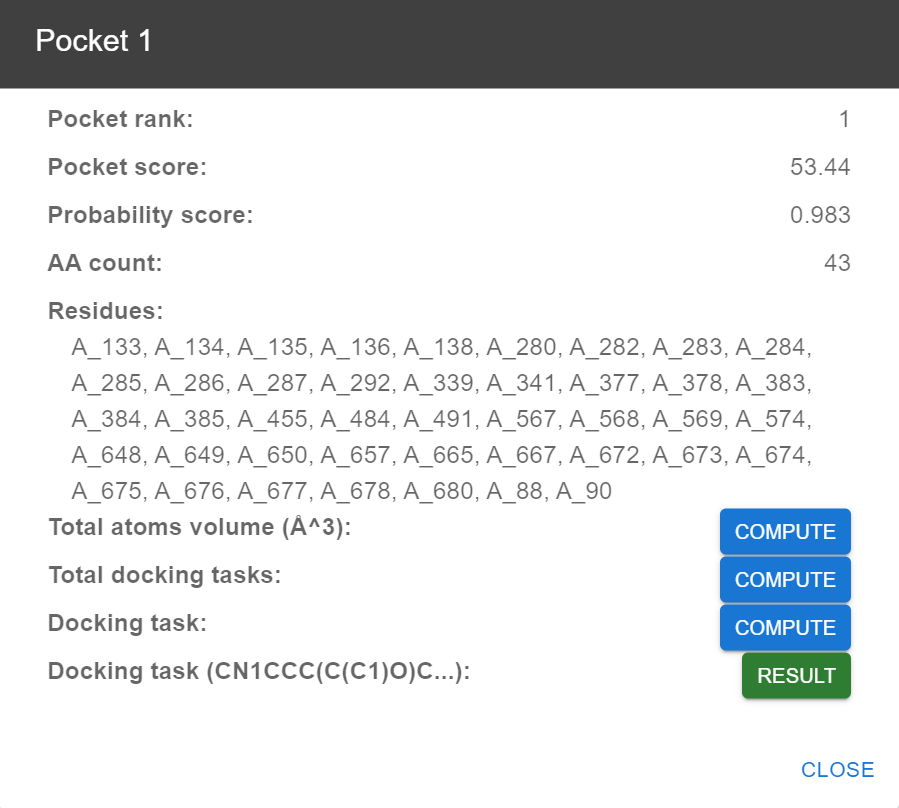
\includegraphics[width=0.75\textwidth]{img/pw_pocketdetails.png}
    \caption{The pocket details dialog component.}
    \label{fig:pocket_details}
\end{figure}

\section{Developer}
\label{sec:developer}

Developers may modify the existing code to their needs. They may edit any of the existing containers described in \cref{sec:prankweb_arch}. One of the expected changes is to implement custom client-side and server-side plug-ins. The following sections describe how to do that.

Before reading the contents of this section, please familiarize yourself with the topic of plug-ins described in \cref{sec:plugins}.

\subsection{Client-side plug-ins}
\label{subsec:dev_client_side}

Implementing custom client-side plug-ins is simple. The creation may be simplified into the following steps:

\begin{enumerate}
    \item Introduce a new task type in the \texttt{frontend/custom-types.ts} file by adding a new value to the \texttt{ClientTaskType} enum.
    \item Create a new \texttt{.tsx} file, preferrably in the \texttt{frontend/tasks} directory.
    \item In this file, implement a method that will compute the task and returns a \texttt{Promise<ClientTaskData>}.
    \item Implement a method that will render the completed task in the dialog window. This method takes the \texttt{ClientTaskData} as an argument and returns a React component - \texttt{JSX.Element}. An example is shown in \cref{lst:code/client-sample-task}.
    \item Optionally, implement saving the computed volumes at least to a hashmap or implement another sort of caching.
    \item Add the new task component anywhere to be rendered. We suggest adding it to the existing dialog window represented by the \texttt{PocketDialogDetails} component. An example is shown in \cref{lst:code/pocket-dialog-details-client-sample}.
\end{enumerate}

\lstinputlisting[language=JavaScript,caption={An example client-side task (in this case referred to as \texttt{frontend/tasks/client-sample-task.tsx}).}, label={lst:code/client-sample-task}]{code/client-sample-task.tsx}

After this implementation, the client-side plug-in is ready to be used.

\lstinputlisting[language=JavaScript,caption={A modified \texttt{PocketDialogDetails} component including the newly introduced client-side plug-in (\texttt{frontend/viewer/components/pocket-dialog-details.tsx}).}, label={lst:code/pocket-dialog-details-client-sample}]{code/pocket-dialog-details-client-sample.tsx}

\subsection{Server-side plug-ins}
\label{subsec:dev_server_side}

Implementing custom server-side plug-ins is more complicated than the client-side ones. Creating a new server-side plug-in consists of the following steps:

\begin{enumerate}
    \item Design a public API for requests.
    \item Add the routes and implement the API in the Flask application.
    \item Create a new Docker container (and possibly volume) for the new plug-in.
    \item Connect the new container to the existing Docker-compose network.
    \item Bind the Celery configuration files to the new container.
    \item Implement the wanted functionality in the Docker container.
    \item Introduce the new server task to the frontend components and enums.
    \item Provide communication between the frontend and the new server-side task via API calls.
\end{enumerate}

Implementing a new server-side plug-in is a complex task and different plug-ins may require different approaches. Therefore, it is highly recommended to have a look at our molecular docking example that is described in detail in \cref{subsec:server-side-plugins} to understand the integration process.
